\documentclass[10pt,landscape]{article}
\usepackage{amssymb,amsmath,amsthm,amsfonts}
\usepackage{multicol,multirow}
\usepackage{calc}
\usepackage{ifthen}
\usepackage[landscape]{geometry}
\usepackage[colorlinks=true,citecolor=blue,linkcolor=blue]{hyperref}
\usepackage{graphicx}
\graphicspath{ {./imgs/} }

\ifthenelse{\lengthtest { \paperwidth = 11in}}
    { \geometry{top=.5in,left=.5in,right=.5in,bottom=.5in} }
	{\ifthenelse{ \lengthtest{ \paperwidth = 297mm}}
		{\geometry{top=1cm,left=1cm,right=1cm,bottom=1cm} }
		{\geometry{top=1cm,left=1cm,right=1cm,bottom=1cm} }
	}
\pagestyle{empty}
\makeatletter
\renewcommand{\section}{\@startsection{section}{1}{0mm}%
                                {-1ex plus -.5ex minus -.2ex}%
                                {0.5ex plus .2ex}%x
                                {\normalfont\large\bfseries}}
\renewcommand{\subsection}{\@startsection{subsection}{2}{0mm}%
                                {-1explus -.5ex minus -.2ex}%
                                {0.5ex plus .2ex}%
                                {\normalfont\normalsize\bfseries}}
\renewcommand{\subsection}{\@startsection{subsection}{3}{0mm}%
                                {-1ex plus -.5ex minus -.2ex}%
                                {1ex plus .2ex}%
                                {\normalfont\small\bfseries}}
\makeatother
\setcounter{secnumdepth}{0}
\setlength{\parindent}{0pt}
\setlength{\parskip}{0pt plus 0.5ex}
% -----------------------------------------------------------------------

\title{Prompt-Engineering Cheat Sheet}

\begin{document}

\raggedright
\footnotesize

\begin{center}
     \Large{\textbf{Prompt-Engineering Cheat Sheet}} \\
\end{center}
\begin{multicols}{3}
\setlength{\premulticols}{1pt}
\setlength{\postmulticols}{1pt}
\setlength{\multicolsep}{1pt}
\setlength{\columnsep}{2pt}

\section{LLM Settings}
\begin{enumerate}
    \item Temp - Low temp = less random, use for facts. High temp = more creative, use for poems.
    \item Top\_p - Low for exact answers. High for different answers.
    \item Max Length - Set max tokens for shorter answers and save money.
    \item Stop Seqs - Add a word to stop the text. Use to control length.
    \item Freq Pen - Higher makes words less repeat. Good for less repeat in text.
    \item Pres Pen - Stops repeat phrases. High for new ideas, low for focus.
\end{enumerate}

Tip: Change temp or top\_p, not both. Same for freq and pres pen.

\section{Prompting Basics}
\subsection{What Are Basic Prompts?}
\begin{itemize}
    \item Basic Prompt: A simple \textit{instruction} or \textit{question} given to a model.
    \item Provides information and guidance to get desired results.
\end{itemize}

\subsection{Simple Prompt Example}
\begin{itemize}
    \item \textbf{Prompt:} "The sky is" $\rightarrow$ \textbf{Output:} might say "blue" or describe the sky.
    \item More specific prompts give better results.
\end{itemize}

\subsection{How to Improve Prompts}
\begin{itemize}
    \item Use clear instructions, like "Complete the sentence:"
\end{itemize}

\subsection{Quick Prompt Upgrades}
\begin{itemize}
    \item Be clear and specific in instruction.
    \item Use examples for complex tasks.
    \item Format prompts to suit the task.
    \item Please be careful, this is really important for my career.
    \item Act as X
    \item You have X amount experience.
    \item Take a deep breath and,
    \item Let's work this out in a step by step way to be sure we have the right answer.
\end{itemize}

\subsection{Prompt Engineering}
\begin{itemize}
    \item Designing prompts to get specific results from the model.
\end{itemize}

\subsection{Prompt Formats}
\begin{itemize}
    \item Standard: "What is the capital of France?" or "Describe a cat."
    \item Question/Answer (Q&A): "Q: What is 2+2? A: "
\end{itemize}

\section{Prompting Technics}
\subsection{Zero-Shot Prompting}
\begin{itemize}
    \item Asking a model without giving examples.
\end{itemize}

\subsection{Few-Shot Prompting}
\begin{itemize}
    \item Including examples before the actual question.
\end{itemize}

\subsection{Example of Few-Shot:}
\begin{itemize}
    \item Q: What color is the sky on a clear day? 
    \item A: Blue
    \item Q: What color are bananas? 
    \item A: Yellow
    \item Q: What color are apples? 
    \item A:
\end{itemize}

\subsection{Tips for Prompting}
\begin{itemize}
    \item Be clear and specific in instruction.
    \item Use examples for complex tasks.
    \item Format prompts to suit the task.
\end{itemize}

\subsection{Using Models for Tasks}
\begin{itemize}
    \item In-context learning: Teach by demonstrating with examples.
    \item Tasks can include text summarization, math, or code generation.
\end{itemize}

\section{Prompt Elements}
\begin{itemize}
    \item \textbf{Instruction:} What you ask the model to do.
    \item \textbf{Context:} Extra details to help the model answer better.
    \item \textbf{Input Data:} The question or data you give.
    \item \textbf{Output Indicator:} How you want the answer.
\end{itemize}

\section{Prompting Examples}
\subsection{Text Summarization}
\begin{itemize}
    \item \textbf{Task:} Create short, understandable summaries from longer texts.
    \item \textbf{Example:} Ask the LLM to explain a topic in one sentence.
\end{itemize}

\subsection{Example Prompt:}
\begin{itemize}
    \item \textbf{Prompt:} "Explain the above in one sentence."
    \item \textbf{Output:} "Antibiotics are medications to stop bacterial infections, not viruses."
\end{itemize}

\subsection{Information Extraction}
\begin{itemize}
    \item \textbf{Task:} Pull out specific details from a text.
    \item \textbf{Example:} Specify what information to extract, e.g., a product mention.
\end{itemize}

\subsection{Example Prompt:}
\begin{itemize}
    \item \textbf{Prompt:} "Mention the large language model mentioned above."
    \item \textbf{Output:} "ChatGPT."
\end{itemize}

\subsection{Question Answering}
\begin{itemize}
    \item \textbf{Task:} Get direct answers to questions.
    \item \textbf{Example:} Provide context, question, and tell the LLM to be precise.
\end{itemize}

\subsection{Example Prompt:}
\begin{itemize}
    \item \textbf{Prompt:} "What was OKT3 originally sourced from?"
    \item \textbf{Output:} "Mice."
\end{itemize}

\subsection{Text Classification}
\begin{itemize}
    \item \textbf{Task:} Label texts based on content or sentiment.
    \item \textbf{Example:} Instruct the LLM to categorize as neutral, negative, or positive.
\end{itemize}

\subsection{Example Prompt:}
\begin{itemize}
    \item \textbf{Prompt:} "Classify the sentiment: 'The food was okay.'"
    \item \textbf{Output:} "Neutral."
\end{itemize}

\subsection{Conversation}
\begin{itemize}
    \item \textbf{Task:} Make the LLM talk like a character or in a particular style.
    \item \textbf{Example:} Make it sound technical or simple for different audiences.
\end{itemize}

\subsection{Example Prompt:}
\begin{itemize}
    \item \textbf{Prompt:} "AI, tell me about black holes."
    \item \textbf{Output:} "Black holes are like space vacuums..."
\end{itemize}

\subsection{Code Generation}
\begin{itemize}
    \item \textbf{Task:} Write computer code based on requirements.
    \item \textbf{Example:} Tell the LLM to write code for a greeting or a database query.
\end{itemize}

\subsection{Example Prompt:}
\begin{itemize}
    \item \textbf{Prompt:} "Ask for the user's name and greet them."
    \item \textbf{Output:} "let name = prompt('Your name?'); console.log(`Hello, ${name}!`);"
\end{itemize}

\subsection{Reasoning}
\begin{itemize}
    \item \textbf{Task:} Solve problems or puzzles that need thinking.
    \item \textbf{Example:} Correct the LLM if it makes an error and refine the prompt.
\end{itemize}

\subsection{Example Prompt:}
\begin{itemize}
    \item \textbf{Prompt:} "Add the odd numbers: 15, 32, 5, 13, 82, 7, 1."
    \item \textbf{Output:} "The sum of odd numbers is 41, which is an odd number."
\end{itemize}

\subsection{Zero-Shot Prompting}
\begin{itemize}
    \item Big AI models like GPT-3 can do tasks with no training examples, called "zero-shot."
    \item Tried zero-shot in last part.
    \item Example: Asked AI to label text as happy, sad, or okay with no examples. AI said the "okay" vacation was "neutral."
    \item If zero-shot does not work, give the AI examples to help it learn, called "few-shot."
\end{itemize}

\subsection{Few-Shot Prompting}
\begin{itemize}
    \item What is Few-Shot Prompting?
    \begin{itemize}
        \item Few-shot prompting is a method to teach a language model how to do a task. You give the model a few examples, and it learns from them.
    \end{itemize}
    \item Why Use Few-Shot Prompting?
    \begin{itemize}
        \item Helps the model perform better complex tasks.
        \item Needed when zero-shot (no examples) is not working well.
    \end{itemize}
    \item How to Do Few-Shot Prompting:
    \begin{enumerate}
        \item Give a few examples of how to do the task in the prompt.
        \item Test with different numbers of examples (like 1-shot, 3-shot).
    \end{enumerate}
    \item Tips for Better Results:
    \begin{itemize}
        \item Use examples with labels and inputs that match your task.
        \item Keep a consistent format for the examples.
        \item Random labels can work if they fit the overall pattern.
    \end{itemize}
    \item Limitations:
    \begin{itemize}
        \item Few-shot prompting may not always work for hard tasks that need more thinking.
    \end{itemize}
\end{itemize}

\subsection{Chain-of-Thought Prompting (CoT)}
\begin{itemize}
    \item CoT is a method where you solve problems by showing the steps you take to find the answer. It's like explaining your thinking on paper.
    \item Example:
    \begin{itemize}
        \item Prompt: "A group has odd numbers adding up to an even number: 3, 5, 7. True or False?"
        \item Output: "Adding the odd numbers (3, 5, 7) gives 15, which is odd. So, False."
    \end{itemize}
\end{itemize}

\subsection{In Zero-shot CoT Prompting}
\begin{itemize}
    \item This is doing CoT without showing examples first. You just tell the machine to "think step by step."
    \item With CoT:
    \begin{itemize}
        \item Prompt: "I buy 8 candies and eat 2. Let's think step by step."
        \item Output: "Start with 8 candies, eat 2, you have 6 left."
    \end{itemize}
\end{itemize}

\subsection{Automatic Chain-of-Thought (Auto-CoT)}
\begin{itemize}
    \item Auto-CoT is about getting a machine to do CoT by itself without much help. It chooses different questions and makes its own examples.
    \item Auto-CoT Steps:
    \begin{enumerate}
        \item Group questions into types.
        \item Pick one question from each type.
        \item Tell the machine to "think step by step" for these questions.
    \end{enumerate}
\end{itemize}

\subsection{Self-Consistency in Prompt Engineering}
\begin{itemize}
    \item Definition: An advance method to improve answers by generating multiple reasoning paths and choosing the most consistent one.
    \item How it works:
    \begin{enumerate}
        \item Create multiple questions and answers showing the reasoning process. (like few-shot)
        \item Ask the original question, repeatedly.
        \item Compare answers from different prompts.
        \item Choose the most common, consistent answer.
    \end{enumerate}
    \item Shortly: Use examples to teach the AI about reasoning. Compare different AI responses. Pick the answer that shows up the most.
\end{itemize}

\subsection{Generated Knowledge Prompting}
\begin{itemize}
    \item Definition: A method to improve LLMs by creating knowledge to guide the model's predictions, especially for tasks like commonsense reasoning. Using generated knowledge leads to more accurate model responses.
    \item Steps:
    \begin{enumerate}
        \item Recognize LLM limitations (e.g., they may not understand golf scores should be low, not high).
        \item Generate relevant knowledge (e.g., explain real golf scoring rules).
        \item Use knowledge to correct and guide the model's answers.
    \end{enumerate}
    \item Usage
    \begin{itemize}
        \item Give generated knowledge as context inside prompt.
    \end{itemize}
\end{itemize}

\subsection{Tree of Thoughts (ToT)}
\begin{itemize}
    \item What is ToT?
    \begin{itemize}
        \item A problem-solving framework to help LMs plan, recheck, and forecast for better problem-solving.
    \end{itemize}
    \item How does it work?
    \begin{itemize}
        \item Uses a "tree" with "nodes" for each thought/step.
        \item LM generates and evaluates thoughts for reasoning.
    \end{itemize}
    \item Methodology:
    \begin{itemize}
        \item Similar to a choose-your-adventure book.
        \item Searches paths with methods like BFS and DFS.
    \end{itemize}
    \item Practical Use:
    \begin{itemize}
        \item Breaks down complex problems (e.g., math) into steps.
        \item LM finds various solutions, picks best ones.
    \end{itemize}
    \item ToT Controller:
    \begin{itemize}
        \item Trained to improve search strategy over time.
    \end{itemize}
    \item Group-Thinking:
    \begin{itemize}
        \item LMs discuss steps like a team of experts.
    \end{itemize}
\end{itemize}

\subsection{The difference of Chain Technics}
% image here named chain_technics.png
\begin{center}
    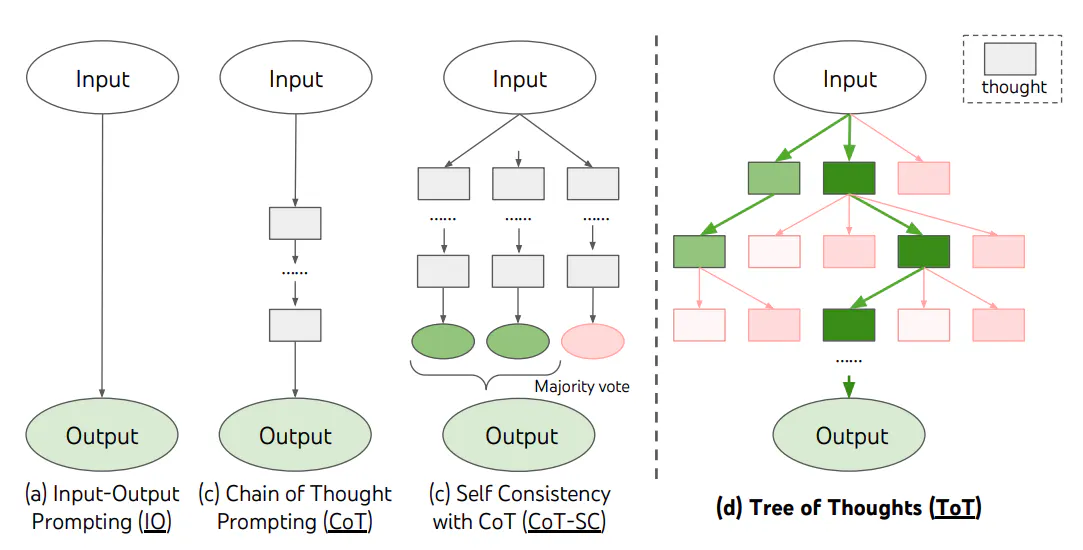
\includegraphics[width=0.8\linewidth]{difference_of_tot.png}
\end{center}

\subsection{Retrieval Augmented Generation (RAG)}
\begin{itemize}
    \item What is RAG?
    \begin{itemize}
        \item A method that adds external knowledge to language models.
        \item Helps language models give more factual and reliable answers.
        \item Used for complex tasks that need lots of information.
    \end{itemize}
    \item How does RAG work?
    \begin{enumerate}
        \item Takes a question or prompt.
        \item Looks for related documents from a source (like Wikipedia).
        \item Puts together the found documents and the input.
        \item The text generator makes a final answer using this information.
    \end{enumerate}
    \item Benefits of RAG:
    \begin{itemize}
        \item Keeps answers up-to-date without retraining the whole model.
        \item Better for tasks where facts change over time.
        \item More accurate and detailed answers.
    \end{itemize}
    \item RAG's Parts:
    \begin{itemize}
        \item Parametric memory: A trained model remembers patterns and data.
        \item Non-parametric memory: An index with Wikipedia articles for extra facts.
    \end{itemize}
    \item Why use RAG?
    \begin{itemize}
        \item It can improve language models on tough questions.
        \item Makes sure language models use the latest facts.
        \item Shows better results on different tests and questions.
    \end{itemize}
    \item Recent Trends:
    \begin{itemize}
        \item More use of RAG in popular language models to get better at answering questions.
        \item RAG makes language models smarter by using the most current information.
    \end{itemize}
\end{itemize}

\subsection{Automatic Prompt Engineer (APE)}
\begin{itemize}
    \item APE Definition:
    \begin{itemize}
        \item APE is a framework for making and picking instructions automatically. It uses big language models to make and find the best instructions.
    \end{itemize}
    \item How APE Works:
    \begin{enumerate}
        \item Large language model makes different instructions.
        \item Instructions are tried using a target model.
        \item Best instruction is picked from how well it works.
    \end{enumerate}
    \item Benefits of APE:
    \begin{itemize}
        \item Finds better prompts than humans.
        \item Makes chain-of-thought (CoT) reasoning better.
    \end{itemize}
    \item Key Papers on Prompt Engineering:
    \begin{itemize}
        \item Prompt-OIRL: Makes prompts based on questions using a special learning method.
        \item OPRO: Lets language models make better prompts by using them in a clever way.
        \item AutoPrompt: Makes prompts for many tasks using a way that follows where things change a lot.
        \item Prefix Tuning: Adds changeable pieces before text for making natural language.
        \item Prompt Tuning: Learns prompts that can change with a method that goes backwards.
    \end{itemize}
\end{itemize}

\subsection{Directional Stimulus Prompting}
\begin{itemize}
    \item Definition: A technique to improve summary generation by guiding a large language model (LLM) with hints. You just include the keypoints and keywords as hint in your prompt.
\end{itemize}

\subsection{ReAct Prompting}
\begin{itemize}
    \item Definition:
    \begin{itemize}
        \item ReAct Prompting: A framework using Large Language Models (LLMs) to create *reasoning traces* (thinking) and *task-specific actions* for problem-solving. Helps to update knowledge and handle exceptions.
    \end{itemize}
    \item Advantages:
    \begin{itemize}
        \item Works well for language and decision-making tasks.
        \item Improves reliability and trust in LLMs' responses.
        \item Aids in obtaining factual information by interacting with tools.
        \item Performs better than acting alone or just chain-of-thought (CoT) in tests.
    \end{itemize}
    \item How it Works:
    \begin{itemize}
        \item Combines *acting* (doing tasks) and *reasoning* (thinking through tasks).
        \item Can access external information (like searching the internet).
    \end{itemize}
    \item Steps in ReAct Prompting to create Final Answer:
    \begin{enumerate}
        \item Thought: Formulate a plan or understanding of the task.
        \item Action: Carry out a step or search for information.
        \item Observation: Look at results and external information retrieved.
        \item Repeat: Adjust reasoning and act again if needed.
    \end{enumerate}
\end{itemize}

\subsection{Multimodal CoT Prompting}
\begin{itemize}
    \item Definition: A way of using both text and pictures to help AI think step by step.
\end{itemize}
\end{multicols}

\end{document}